\documentclass[a4paper, 10pt]{article}
\usepackage[utf8]{inputenc}
\usepackage{graphicx}
\title{\bf CC0402 - Programação Orientada a Objetos}
\author{Gabriel de Sousa Lima}
\date{Abril 2019}

\begin{document}

\maketitle

\section{Introdução}
\ A programação orientada a objetos é um modelo de análise, projeto e programação 
de software baseado na composição e interação entre diversas unidades
chamadas de "objetos".A POO (Programação Orientada a Objetos) é um dos 4
principais paradigmas de programação (as outras são programação imperativa, funcional e lógica).\\
Os principais tópicos são: \\
Conceitos básicos: classes, objetos, mensagens, encapsulamento, herança, polimorfismo. \\
Programação orientada a objetos utilizando uma linguagem de programação orientada a objetos. ~\cite{wiki} \\
Análise e projeto orientados a objetos. UML. Padrões de projeto de software. \\
POO se insere na área de Linguagem de Programação. ~\cite{Kurt}
\begin{figure}[!htb]
    \center{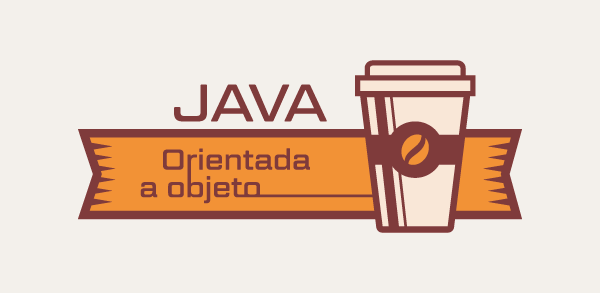
\includegraphics[width=0.5\textwidth]{artigo_programacao-orientada-a-objetos-com-java_18449.png}}
    \caption{\label{fig:my-label} Java. Uma das linguagens mais famosas relacionada a Orientação de Objetos.}
\end{figure}

\section{Relevância}
\ O paradigma "orientado ao objeto" tem origem nos estudos da cognição e influenciou a inteligência artificial e a linguística, dada a relevância para a abstração de conceitos do mundo real.
\\ Porque é tão importante?
\\ "Hoje em dia, o mercado de programação é dominado pelo paradigma orientado a objetos." ~\cite{Jackson}
\\
\\
\\
\section{Relação com Outras Disciplinas}
\begin{table}[!htb]

\begin{tabular}{|l|l|}
\hline
CC0503 - Banco de Dados         & \begin{tabular}[c]{@{}l@{}}Utiliza os dados como unidade básica\\ para construção do programa.\end{tabular} \\ \hline
CC0603 - Engenharia de Software & \begin{tabular}[c]{@{}l@{}}Pois é um dos 4 principais paradigmas\\ da programação.\end{tabular}             \\ \hline
\end{tabular}
\end{table}

\bibliographystyle{ieeetr}
\bibliography{Gabriel_de_Sousa_Lima.bib}

\end{document}
